\documentclass[10pt]{beamer}
\usefonttheme{professionalfonts,serif}

\def\newblock{\hskip .11em plus .33em minus .07em}

\usepackage[numbers,sort]{natbib}
\renewcommand{\rmdefault}{psbx}

\usepackage[utf8]{inputenc}
\usepackage[T1]{fontenc}
\usepackage{textcomp}

\usepackage{eulervm}

\usetheme{default}           % tips from David Blei
\useinnertheme{circles}
\useoutertheme{infolines}
\setbeamertemplate{headline}{}
\setbeamertemplate{navigation symbols}{}
\setbeamerfont{itemize/enumerate subbody}{size=\normalsize}
\setbeamerfont{itemize/enumerate subsubbody}{size=\normalsize}
\usecolortheme{seahorse}
\setbeamersize{text margin left=2mm,text margin right=2mm}
\usepackage{media9}
\newcommand{\Red}{\textcolor{red}}
\newcommand{\Blue}{\textcolor{blue}}
\definecolor{mypine}{rgb}{0.05,0.45,0.05}
\newcommand{\Green}{\textcolor{mypine}}
\newcommand{\y}{y}
\newcommand{\z}{z}

\setlength{\parskip}{1em}

\title[The EM algorithm]{The Expectation Maximization\\ or EM algorithm}
\author{Carl Edward Rasmussen}
\date{November 15th, 2017}

\begin{document}

\begin{frame}
\titlepage

\end{frame}

\begin{frame}
\frametitle{Contents}

\begin{itemize}
\item notation, objective
\item the lower bound functional, ${\cal F}(q(H),\theta)$
\item the EM algorithm
\item example: Gaussian mixture model
\item Appendix: KL divergence
\end{itemize}
\end{frame}

\begin{frame}
\frametitle{Notation}

Probabilistic models may have \emph{visible} (or \emph{observed}) variables $\y$, \emph{latent} variables, (or \emph{hidden} or \emph{unobserved}  variables or \emph{missing data}) $\z$ and parameters $\theta$.

{\bf Example}: in a Gaussian mixture model, the visible variables are the observations, the latent variables are the assignments of data points to mixture components and the parameters are the means, variances, and weights of the mixture components.

The likelihood, $p(\y|\theta)$, is the probability of the visible variables given the parameters. The goal of the EM algorithm is to find parameters $\theta$ which maximize the likelihood. The EM algorithm is iterative and converges to a local maximum.

Throughout, $q(\z)$ will be used to denote an arbitrary distribution of the latent variables, $\z$. The exposition will assume that the latent variables are continuous, but an analogue derivation for discrete $\z$ can be obtained by substituting integrals with sums.
\end{frame}

\begin{frame}
\frametitle{The lower bound}

Bayes' rule:
\[
p(\z|\y,\theta)\;=\;\frac{p(\y|\z,\theta)p(\z|\theta)}{p(\y|\theta)}\;\;\Leftrightarrow\;\;
p(\y|\theta)\;=\;\frac{p(\y|\z,\theta)p(\z|\theta)}{p(\z|\y,\theta)}.
\]
Multiply and divide by an arbitrary (non-zero) distribution q(\z):
\[
p(\y|\theta)\;=\;\frac{p(\y|\z,\theta)p(\z|\theta)}{q(\z)}\;\frac{q(\z)}{p(\z|\y,\theta)},
\]
take logarithms:
\[
\log p(\y|\theta)\;=\;\log\frac{p(\y|\z,\theta)p(\z|\theta)}{q(\z)}\;+\;\log\frac{q(\z)}{p(\z|\y,\theta)},
\] 
and average both sides wrt $q(\z)$:
\[
\log p(\y|\theta)\;=\;\underbrace{\Blue{\int q(\z)\log\frac{p(\y|\z,\theta)p(\z|\theta)}{q(\z)}d\z}}_{\text{lower bound functional\ }\Blue{{\cal F}(q(\z),\theta)}}\;+\;
\underbrace{\Red{\int q(\z)\log\frac{q(\z)}{p(\z|\y,\theta)}d\z}}_{\!\!\!\!\!\!\!\!\!\!\!\text{non-negative\ }\Red{{\cal KL}(q(\z)|\!|p(\z|\y,\theta)\!)}}.
\]
\end{frame}

\begin{frame}
\frametitle{The EM algorithm}

From initial (random) parameters $\theta^{t=0}$ iterate $t=1,\ldots,T$ the two steps:

{\bf E step}: for fixed $\theta^{t-1}$, maximize the lower bound $\Blue{{\cal F}(q(\z),\theta^{t-1})}$ wrt $q(\z)$. Since the log likelihood $\log p(\y|\theta)$ is independent of $q(\z)$ maximizing the lower bound is equivalent to minimizing $\Red{{\cal KL}(q(\z)||p(\z|\y,\theta^{t-1}))}$, so $\Green{q^t(\z)=p(\z|\y,\theta^{t-1})}$.

{\bf M step}: for fixed $q^t(\z)$ maximize the lower bound $\Blue{{\cal F}(q^k(\z),\theta)}$ wrt $\theta$. We have:
\[
\Blue{{\cal F}(q(\z),\theta)}\;=\;\int q(\z)\log\big(p(\y|\z,\theta)p(\z|\theta)\!\big)d\z-\int q(\z)\log q(\z)d\z,
\]
whose second term is the entropy of $q(\z)$, independent of $\theta$, so the M step is
\[
\Green{\theta^t\;=\;\underset{\theta}{\rm argmax}\int q^t(\z)\log\big(p(\y|\z,\theta)p(\z|\theta)\!\big)d\z.}
\]
Although the steps work with the lower bound, each iteration cannot decrease the log likelihood as
\[
\log p(\y|\theta^{t-1})\;\overset{\Green{\rm E\ step}}{\!\!\!\!\!\!\phantom{\leq}=}\;\Blue{{\cal F}(q^t(\z),\theta^{t-1})}\;
\overset{\Green{\rm M\ step}}{\leq}\;\Blue{{\cal F}(q^t(\z),\theta^t)}\;
\overset{{\rm lower\ bound}}{\leq}\log p(\y|\theta^t).
\]
\end{frame}


\begin{frame}
\frametitle{EM as Coordinate Ascent in ${\cal F}$}

\centerline{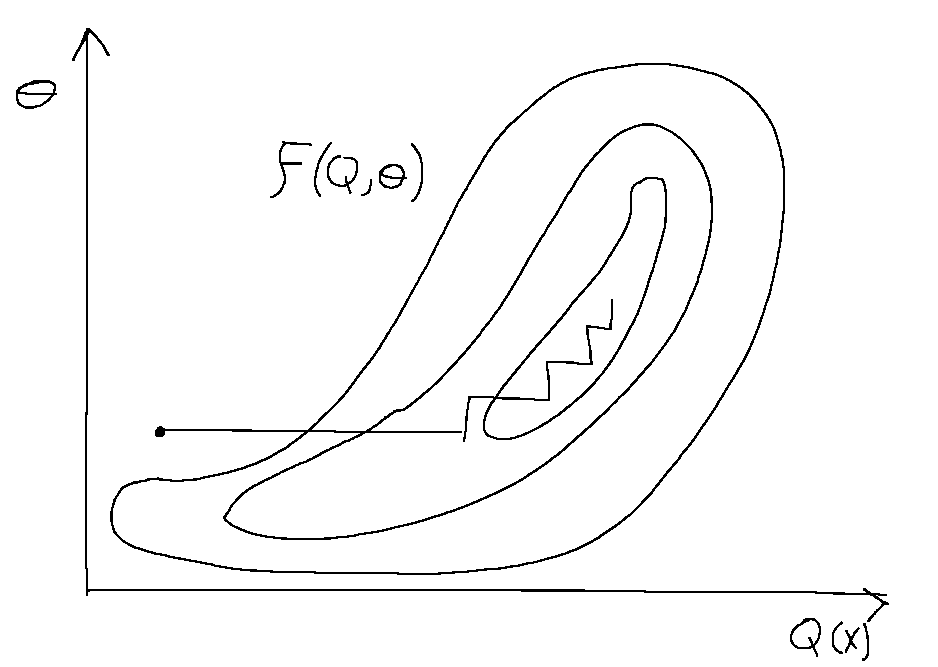
\includegraphics[width=100mm]{fqtheta}}
\end{frame}



\begin{frame}
\frametitle{Example: Mixture of Gaussians}

In a Gaussian mixture model, the parameters are $\theta=\{\mu_j,\sigma_j^2,\pi_j\}_{j=1\ldots k}$ the mixture
means, variances and mixing proportions for each of the $k$ components. There is one latent variable per data-point $\z_i, i=1\ldots n$ taking on values $1\ldots k$.

The probability of the observations given the latent variables and the parameters, and the prior on latent variables are
\[
p(y_i|\z_i=j,\theta)\;=\;
\exp\big(\!-\tfrac{(y_i-\mu_j)^2}{2\sigma^2_j}\big)/\sqrt{2\pi\smash{\sigma^2_j}},\qquad p(\z_i=j|\theta)\;=\;\pi_j,
\]
so the E step becomes:
\[
q(\z_i=j)\;\propto\;u_{ij}=\pi_j\exp(-(y_i-\mu_j)^2/2\sigma^2_j)/\sqrt{2\pi\smash{\sigma_j^2}}
\;\Rightarrow\;q(\z_i=j)=\Green{r_{ij}}=\frac{u_{ij}}{u_i},
\]
where $u_i=\sum_{j=1}^ku_{ij}$. This shows that the posterior for each latent variable, $\z_i$ follows a discrete distribution with probability given by the product of the prior and likelihood, renormalized. Here, $\Green{r_{ij}}$ is called the \emph{\Green{responsibility}} that component $j$ takes for data point $i$.
\end{frame}

\begin{frame}
\frametitle{Example: Mixture of Gaussians continued}

The \Blue{lower bound} is
\[
\Blue{{\cal F}(q(\z),\theta)}\;=\;\sum_{i=1}^n\sum_{j=1}^k\!q(\z_i=j)
\big[\log(\pi_j)-\tfrac{1}{2}(\y_i-\mu_j)^2/\sigma_j^2-\tfrac{1}{2}\log(\sigma_j^2)\big]+{\rm const}.
\]
The M step, optimizing $\Blue{{\cal F}(q(\z),\theta)}$ wrt the parameters, $\theta$
\[
\begin{split}
\frac{\partial\Blue{{\cal F}}}{\partial\mu_j}\;=\;
\sum_{i=1}^n\!q(\z_i=j)\frac{\y_i-\mu_j}{\sigma_j^2}\;=\;0\;\Rightarrow\;
\mu_j&=\frac{\sum_{i=1}^n\!q(\z_i=j)\y_i}{\sum_{i=1}^n\!q(\z_i=j)},\\
\frac{\partial\Blue{{\cal F}}}{\partial\sigma^2_j}\;=\;
\sum_{i=1}^n\!q(\z_i=j)\big[\frac{(\y_i-\mu_j)^2}{2\sigma_j^4}-\frac{1}{2\sigma_j^2}\big]=0
\;\Rightarrow\;\sigma_j^2&=\frac{\sum_{i=1}^n\!q(\z_i=j)(\y_i-\mu_j)^2}{\sum_{i=1}^n\!q(\z_i=j)},\\
\frac{\partial[\Blue{{\cal F}}+\lambda(1-\sum_{j=1}^k\pi_j)]}{\partial\pi_j}=0
\;\Rightarrow\;\pi_j&=\frac{1}{n}\sum_{i=1}^n\!q(\z_i=j),
\end{split}
\]
%
which have nice interpretations in terms of \Blue{weighted averages}.
\end{frame}


\begin{frame}
\frametitle{Clustering with MoG}

\centerline{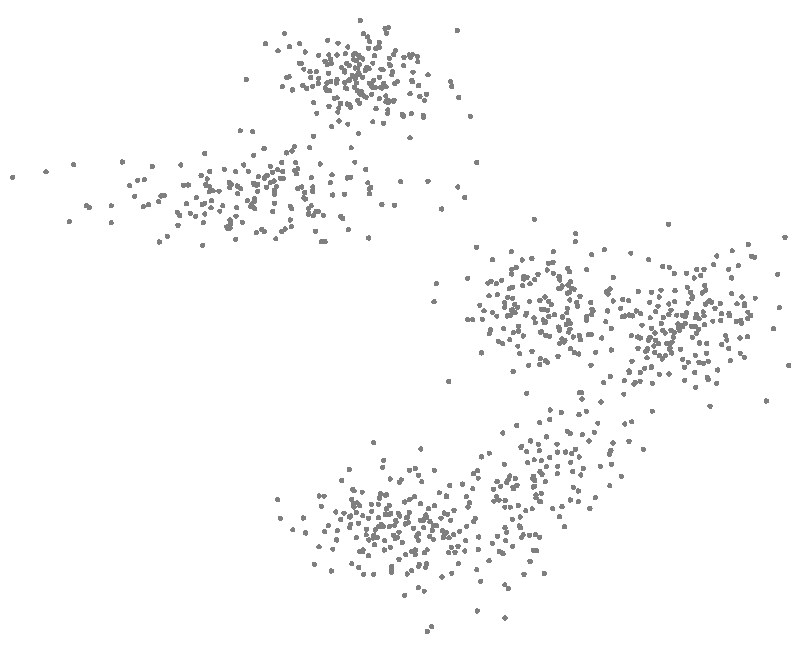
\includegraphics[height=0.85\textheight]{mog-cluster-data}}
\end{frame}

\begin{frame}
\frametitle{Clustering with MoG}

\centerline{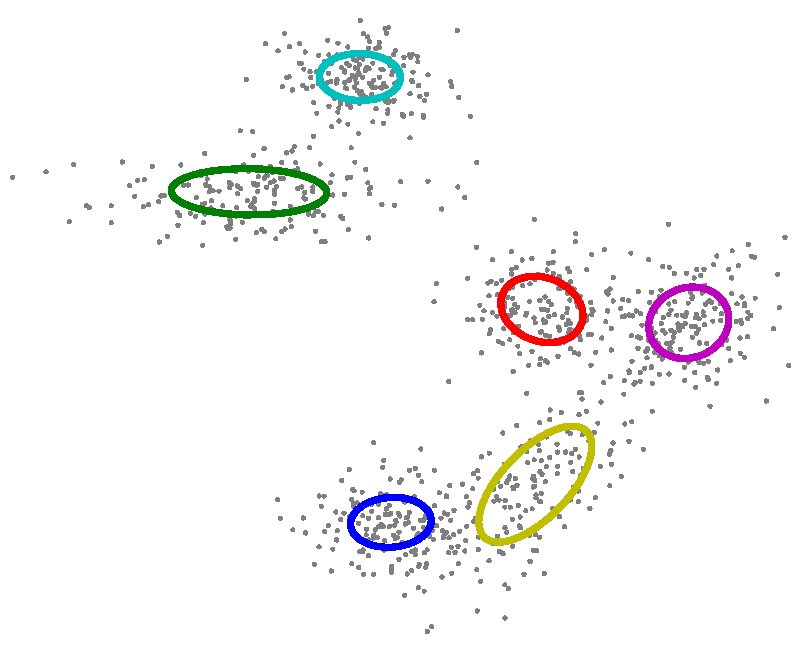
\includegraphics[height=0.85\textheight]{mog-cluster-ellipses}}
\end{frame}


\begin{frame}
\frametitle{Appendix: some properties of KL divergence}

The (asymmetric) Kullbach Leibler divergence (or relative entropy) ${\cal KL}(q(x)||p(x))$ is non-negative. To minimize, add a Lagrange multiplier enforcing proper normalization and take variational derivatives:
\[
\frac{\delta}{\delta q(x)}\Big[\int q(x)\log\frac{q(x)}{p(x)}dx+\lambda\big(1-\int q(x)dx\big)\Big]\;
=\;\log\frac{q(x)}{p(x)}+1-\lambda.
\]
Find stationary point by setting the derivative to zero:
\[
q(x)\;=\;\exp(\lambda-1)p(x),\text{\ \ normalization conditon\ }\lambda\;=\;1, \text{\ \ so\ }q(x)\;=\;p(x),
\]
which corresponds to a minimum, since the second derivative is positive:
\[
\frac{\delta^2}{\delta q(x)\delta q(x)}{\cal KL}(q(x)||p(x))\;=\;\frac{1}{q(x)}\;>\;0.
\]
The minimum value attained at $q(x)=p(x)$ is ${\cal KL}(p(x)||p(x))=0$, showing that 
${\cal KL}(q(x)||p(x))$
\begin{itemize}
\item is non-negative
\item attains its minimum 0 when $p(x)$ and $q(x)$ are equal (almost everywhere).
\end{itemize}
\end{frame}

\end{document}